 
\chapter{METODOLOGÍA}

Para poder realizar esta investigación, primero se realizó una apropiación de 
conocimiento y se definió el marco conceptual sobre el cual se iba a realizar el proyecto. Primero fue importante 
entender el problema que se desarrollaría, identificando los patrones en objetos en movimiento, 
para posteriormente enfocarse en los patrones de agrupamiento conocidos como ``flocks''.

Se compararon dos algoritmos, BFE y LCMFlock propuestos por \cite{VieiraT13} y \cite{turdu2014}, con el fin de
identificar los problemas asociados a su rendimiento. Se escogió únicamente estos dos algoritmos 
para la comparación debido a que este análisis se enfocaría únicamente a patrones de agrupamiento 
(flocks) y estos son los algoritmos más representativos que existen hasta
el momento en este campo. 

Para realizar esta comparación se implementaron los algoritmos BFE y LCMFLOCK basados en el 
pseudo-código publicado por \cite{vieira2009line}  y \cite{romero2011mining} respectivamente,
usando Python versión 3 debido a la facilidad y comodidad para el programador. 
Realizar esta implementación tenía como objetivo hacer una inspección más detallada de cada 
algoritmo y de las estructuras utilizadas en la implementación con el fin de encontrar
sus inconvenientes y buscar una mejora. El código fuente se  puede descargar
desde el repositorio del proyecto \footnote{Repositorio del proyecto: 
\url{https://github.com/poldrosky/FPFlock}}.

A continuación se describen los detalles de la implementación de los algoritmos BFE y LCMFlock.

\section{IMPLEMENTACIÓN DE BFE}

Este algoritmo se divide en dos partes: la primera parte, encontrar los discos 
dado un radio ($\epsilon$) y un número mínimo de puntos ($\mu$) para cada instante de tiempo. La 
segunda parte, encontrar
el número de puntos que permanecen juntos (flocks) durante un rango de tiempo ($\delta$).

Para la primera parte es necesaria la utilización tanto de diccionarios de datos como
estructuras kd-tree para la búsqueda del vecino más cercano, en esta implementación se usó la clase 
scipy.spatial.cKDTree de
SciPy \footnote{Scipy es un ecosistema basado en Python, software de código abierto para las 
matemáticas, la ciencia y la ingeniería.
\url{http://www.scipy.org/}} la cual proporciona  un índice dentro de un conjunto de puntos 
k-dimensionales que se pueden utilizar
para buscar rápidamente los vecinos más cercanos de cualquier punto. 

Para realizar este proceso de implementación fue de gran utilidad el uso del software QGIS, un 
sistema de información geográfica libre y de código abierto disponible en \cite{QGISsoftware}, 
debido a que la primera parte del algoritmo esta basada en encuentrar de los discos máximos, se 
utilizo QGIS para realizar pruebas unitarias a medida que se avanzaba en las etapas de 
depuración, como lo muestra la figura~\ref{fig:findMaximalDisk}.

\begin{figure*}
  \centering
  \subfigure[Todos los discos]{\label{b1} 
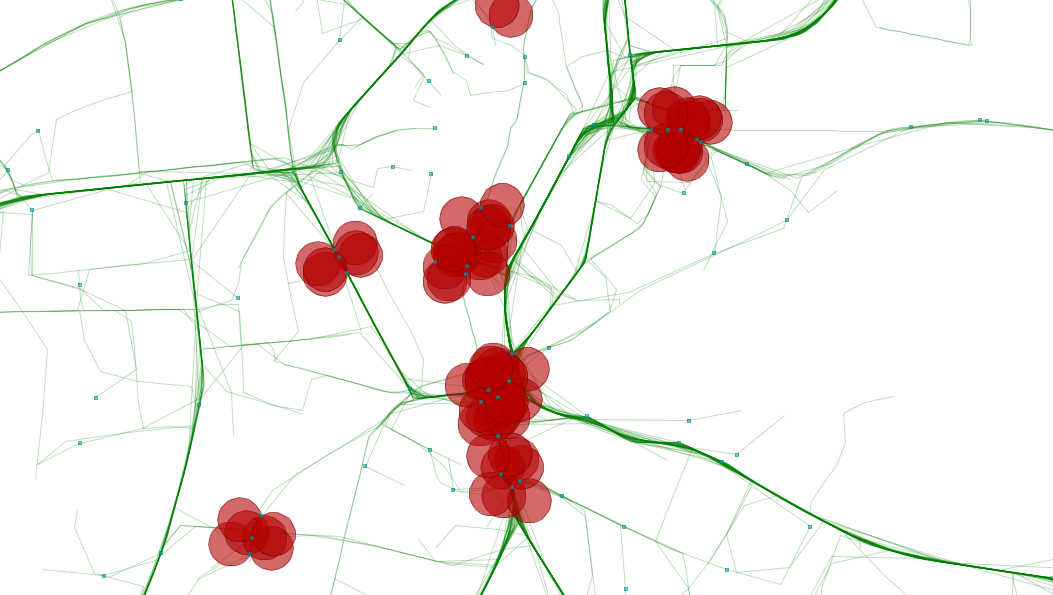
\includegraphics[scale=0.3]{pictures/bfe1.png}}
  \subfigure[Discos que cumplen $\mu$ mínimo]{\label{b2} 
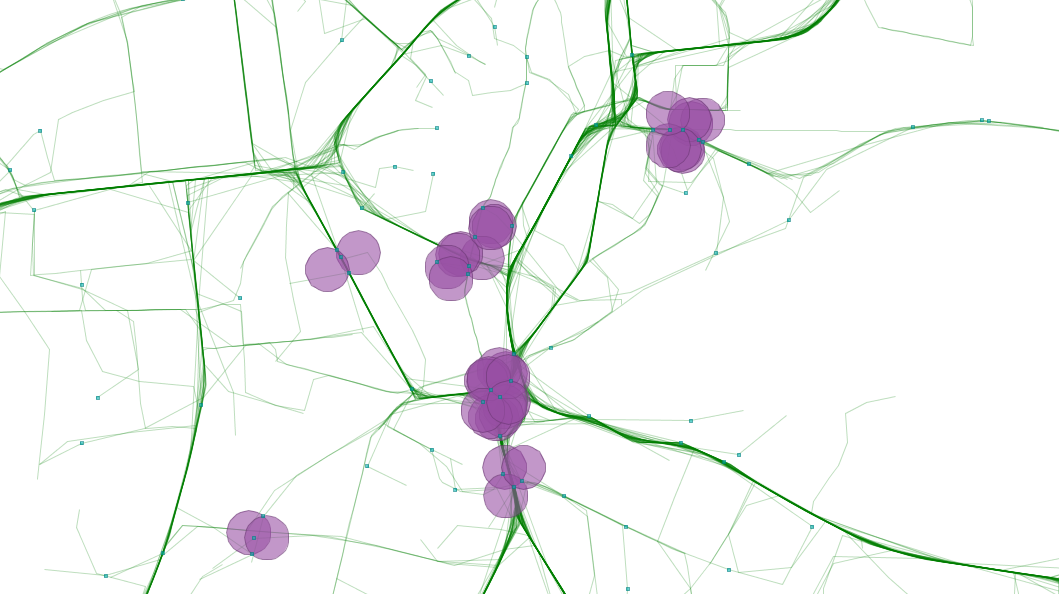
\includegraphics[scale=0.3]{pictures/bfe2.png}}
\subfigure[Discos máximos]{\label{b3} 
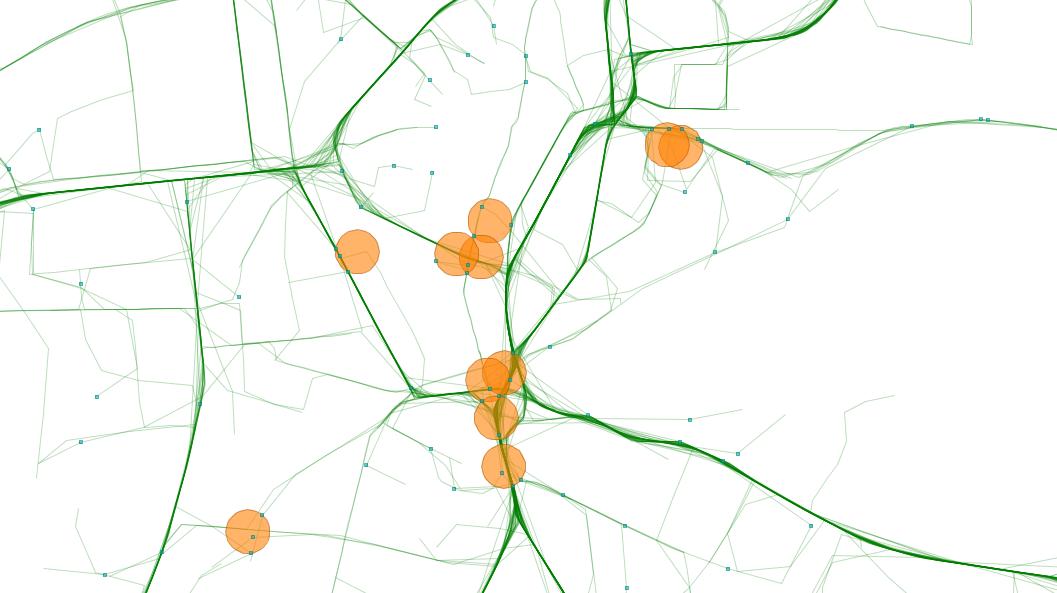
\includegraphics[scale=0.3]{pictures/bfe3.png}}
  \caption{Proceso para encontrar los discos máximos \cite{romero2011mining}.}
  \label{fig:findMaximalDisk}
\end{figure*}


Los conjuntos de discos para 
cada instante de tiempo se almacenaron en diccionarios los cuales fueron combinados en la segunda 
parte del algoritmo.  Finalmente, se almacenaron en una base de datos los flocks que cumplían los 
parámetros solicitados.  Para cada flock se almacenó un arreglo con los objetos que pertenecen a 
dicho flock, y los tiempos de inicio y final para cada caso.


\section{IMPLEMENTACIÓN DE LCMFLOCK}

Este algoritmo usa la primera parte del algoritmo de BFE para encontrar los discos. En la segunda 
parte, para abordar el problema
de combinatoria utiliza un enfoque de patrones frecuentes, en el cual se construyó un 
diccionario de datos asociando la localización 
de los puntos de cada trayectoria con su respectivo disco generado una versión transaccional del 
conjunto de datos. En la figura~\ref{fig:transactionTrajectory}, se muestra como se realiza conversión de las trayectorias en  
transacciones. Este conjunto
es pasado como parámetro, junto con el  número mínimo de puntos ($\mu$), al algoritmo 
LCM\cite{uno2004lcm}, disponible para descargar en \cite{FIMIHomep}.

\begin{figure*}
  \centering
  \subfigure[\cite{romero2011mining}]{ 
  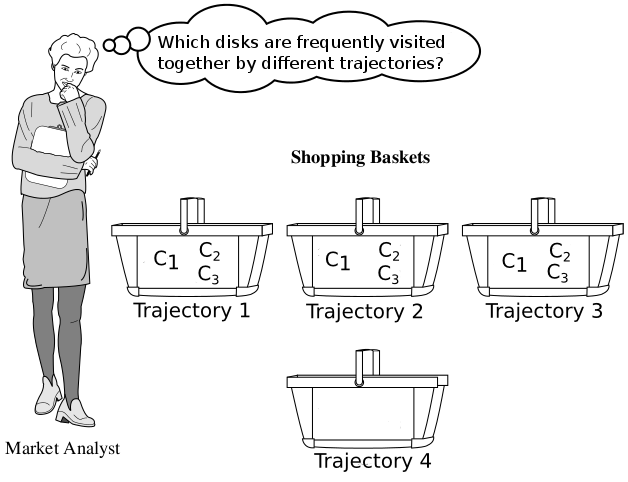
\includegraphics[scale=0.5]{pictures/lcm2.png}}
  \subfigure[\cite{vieira2009line}]{
  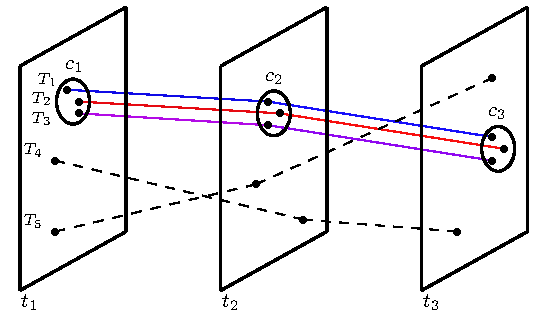
\includegraphics[scale=0.8]{pictures/flock_example.pdf}}
  \caption{Ejemplos de patrones frecuentes en trayectorias.}
  \label{fig:transactionTrajectory}
\end{figure*}

 Aquí se encuentran disponibles dos variantes del programa; LCM\_max y LCM\_closed los cuales 
recuperarán el conjunto de patrones máximo y cerrado\cite{han2000mining}.  LCMFLOCK utiliza el 
concepto de patrones máximos y cerrados para identificar los patrones de agrupamiento de mayor 
duración.  De esta manera, el parámetro $\delta$ se utiliza solo para filtrar aquellos patrones que 
no cumplan con este parámetro \cite{romero2011mining}.
 
 La salida de LCM es un archivo de texto, donde cada línea es un patrón que contiene un conjunto de 
ID's de discos separados por espacios que representan los patrones de agrupamiento (flocks). Sin 
embargo, se requiere de un análisis posterior para verificar que dichos discos ocurran en tiempos 
consecutivos.  De cada patrón, se extraen los objetos que encierra cada disco así como los tiempos 
de inicio y final los cuales son almacenados en una base de datos.
 
\section{VALIDACIÓN}
 
 Para poder validar la correcta implementación de los algoritmos se siguió una metodología similar a 
la propuesta en \cite{benkert2008reporting}. Se crearon conjuntos de datos sintéticos a los cuales 
se les insertó aleatoriamente un número específico de trayectorias y flocks. La 
tabla~\ref{tab:validacion}, relaciona los conjuntos de datos construidos y con los cuales los 
algoritmos fueron validados.  Una copia de los conjuntos de datos y el script utilizado para la 
validación está disponible en el repositorio del proyecto \footnote{Conjuntos de prueba: 
\url{https://github.com/poldrosky/FPFlock/tree/master/Src/Datasets/}}. El total de flocks insertados 
en cada caso fueron correctamente descubiertos por las dos implementaciones.
 
\begin{table}
\caption{Conjunto de datos validación}
\label{tab:validacion}
\centering
\scalebox{0.8}{
\begin{tabular}{c c r r c}
\toprule
\multirow{2}{*}{Dataset}& \multirow{2}{*}{Red}& \multicolumn{1}{c}{Número de}& Número de  & 
Instantes de\\
                        &                         & Trayectorias & \multicolumn{1}{c}{Flocks} & 
tiempo\\
\midrule
SJ5000T100t100f  & Sintética & 5000 & 100 & 100 \\
SJ5000T100t200f	& Sintetica & 5000 & 200 & 100 \\
SJ5000T100t300f	& Sintetica & 5000 & 300 & 100 \\
SJ5000T100t400f	& Sintetica & 5000 & 400 & 100 \\
SJ5000T100t500f	& Sintetica & 5000 & 500 & 100 \\
SJ2500T100t500f  & Sintética & 2500 & 500 & 100  \\
SJ7500T100t500f  & Sintética & 7500 & 500 & 100  \\
SJ10000T100t500f  & Sintética & 10000 & 500 & 100  \\
SJ12500T100t500f  & Sintética & 12500 & 500 & 100  \\
SJ15000T100t500f  & Sintética & 15000 & 500 & 100  \\
SJ17500T100t500f  & Sintética & 17500 & 500 & 100  \\
SJ20000T100t500f  & Sintética & 20000 & 500 & 100  \\
\bottomrule
\end{tabular}}\par
\bigskip
\end{table}

\section{ANÁLISIS DE BFE y LCMFLOCK}

Se realizó un análisis de desempeño entre los algoritmos de BFE y LCMFLlock, usando varios 
conjuntos de prueba, este análisis se puede detallar en \cite{cabrera}. Algunas de las 
conclusiones de este análisis, fueron:

\begin{itemize}
\item Las estructuras de tipo árbol, y en específico, los kd-tree presentaron los mejores 
resultados. Esto se configura
como un aspecto clave para la búsqueda del conjunto final
de discos para cada instante de tiempo. 

 \item Aunque el proceso de identificación de los discos en cada
instante de tiempo es compartido por ambos algoritmos, el
proceso de combinación es mucho más eficiente utilizando
un enfoque basado en técnicas de patrones frecuentes.

\item Aunque LCMFLock presenta mejores resultados, este
aún se ve afectado por el proceso de identificación de los
discos. El número de discos a evaluar crece exponencialmente a medida que crece el valor $\varepsilon$ de y la 
densidad de puntos dentro del conjunto.

\item En BFE, el reporte de flocks es demasiado alto en
comparación con LCMFlock. BFE separa los
flocks de acuerdo al parámetro $\delta$ en procura de limitar
el número de discos a comparar. Esto dificulta la interpretación de resultados ya que es necesario 
de un análisis adicional para encontrar los flocks más largos a partir de
aquellos con una duración fija. En LCMFlock esto se
soluciona con el uso del algoritmo LCM para la detección
de patrones máximos y cerrados.

\item La capacidad de encontrar los flocks más largos ciertamente es una ventaja de LCMFlock sobre 
BFE. Sin embargo, LCMFlock, a diferencia de BFE, requiere de
una ventana fija de tiempo donde será aplicado lo que
le impide reportar patrones en tiempo real. 
\end{itemize}

Debido a este análisis realizado el algoritmo propuesto, presentado en el siguiente capítulo se 
enfocó en resolver dos problemas claves: mejorar el desempeño
durante la búsqueda de los discos e implementar mecanismos de detección en tiempo real.




